\documentclass[12pt,a4paper]{amsart}

\title{Products and Moebius Functions}

\usepackage[euler-digits]{eulervm}
\usepackage{geometry}
\usepackage{amssymb} % \rtimes
\usepackage{graphicx} % \scalebox
\usepackage{mathtools} % \mathclap
\usepackage{tikz}

\let\SS\relax
\newcommand{\SS}{\mathcal{S}}
\newcommand{\Q}{\mathbb{Q}}
\newcommand{\Sub}{\mathsf{Sub}}
\newcommand{\Size}[1]{\left|#1\right|}
\newcommand{\ximes}{\tilde{*}^{\kappa}}
\renewcommand{\gcd}{\mathsf{gcd}}
\newcommand{\lcm}{\mathsf{lcm}}

\newtheorem{theorem}{Theorem}[section]
\newtheorem{corollary}[theorem]{Corollary}

\newcommand{\kstar}{\mathbin{\scalebox{0.61}{$\boxtimes$}}}
\newcommand{\kstarhat}{\mathbin{\hat{\scalebox{0.61}{$\boxtimes$}}}}
\newcommand{\kstartilde}{\mathbin{\tilde{\scalebox{0.61}{$\boxtimes$}}}}

\begin{document}

\maketitle

\section{Idempotents in the Burnside Ring}

[Reference: Gluck]

The Burnside ring $B(G)$ has two natural basis, one in correspondence
to the (isomorphism types of) transitive $G$-sets,
\begin{align*}
  u_K : H \mapsto |(G/K)^H|, \quad K, H \leq G
\end{align*}
(note that $u_K = u_{K'}$ iff $K$ and $K'$ are conjugate in $G$), and
one consisting of idempotents
\begin{align*}
e_H \colon K \mapsto [K \sim_G H],  \quad H \leq G
\end{align*}
(again with
$e_H = e_{H'}$ iff $H$ and $H'$ are conjugate in $G$).
In order to express the $e_H$ in terms of the $u_K$,
we first express $u_K$ in terms of the $e_H$ and then
apply Moebius inversion.  The general principle is
\begin{align*}
  g(x, z) = \sum_y \zeta(x, y) f(y, z) \iff
  f(x, z) = \sum_y \mu(x, y) g(y, z),
\end{align*}
where $\zeta(x, y) = [x \leq y]$ is the incidence function/matrix
of the partial order $\leq$, and $\mu$ is the corresponding Moebius
function, the matrix inverse of $\zeta$. Or, in the one-parameter case:
\begin{align*}
    g(x) = \sum_y \zeta(x, y) f(y) \iff
  f(x) = \sum_y \mu(x, y) g(y).
\end{align*}

Now,
\begin{align*}
  u_K(H) &= \Size{N_G(K) : K} \cdot \# \{K^a \geq H : a \in G\} \\
           &= \Size{N_G(H)} \Size{K}^{-1}
             \cdot \# \{H^a \leq K : a \in G\},
\end{align*}
whence
\begin{align*}
  \Size{K} u_K = \sum_H \zeta(H, K) \Size{N_G(H)} e_H.
\end{align*}
Moebius inversion yields
\begin{align*}
  \Size{N_G(H)} e_H
  =
  \sum_K \mu(K, H)
  \Size{K} u_K.
\end{align*}

\section{Lambda}

Recall $(A, B) \leq_{P/K} (C, D)$ if
$A \leq C$, $B \leq D$, and $\phi \colon Ab \mapsto Cb$ is an isomorphism
from $A/B$ to $C/D$.
For $A \unlhd P \leq G$, define
\begin{align*}
  \lambda^P_A := \sum_{(Q, B)} \mu (Q, P) \Size{B},
\end{align*}
where $\mu$ is the Moebius function of the poset
$\{ (Q, B) : Q/B \cong P/A \}$, partially ordered with respect to
$\leq_{P/K}$. Note that $\mu((Q, B), (P, A)) = \mu(Q, P)$ in the
set of subgroups $\{Q \leq P : QA = P \}$.

By Moebius inversion,
\begin{align*}
  \Size{B} = \sum_{(P, A)} \zeta(P, Q) \lambda^P_A,
\end{align*}
where $\zeta(P, A) = [(P, A) \leq_{P/K} (Q, B)]$.
In particular, if $(P, A)$ is \emph{minimal} with respect to $\leq_{P/K}$
(which is the case exactly when $A \leq \Phi(P)$) then
$\lambda^P_A = \Size{A}$.

Now the class incidence matrix $M$ has entries
\begin{align*}
  m_{(P, A), (Q, B)} = \# \{ (P, A)^a \geq (Q, B) : a \in G \}.
\end{align*}
We have
\begin{align*}
  \Size{G: N_G(Q, B)} m_{(P, A), (Q, B)} =
  \Size{G: N_G(P, A)}  \# \{ (Q, B)^a \leq (P, A) : a \in G \},
\end{align*}
so that
\begin{align*}
  \Size{N_G(Q, B)} \Size{N_G(P, A)}^{-1} m_{(Q, B), (P, A)} =  \# \{ (P, A)^a \leq (Q, B) : a \in G \}
\end{align*}
Classwise:
\begin{align*}
  \Size{B} &= \sum_{[P, A]} \# \{ (P, A)^a \leq (Q, B) : a \in G \}\, \lambda^P_A \\
\Size{N_G(Q, B)}^{-1} \Size{B}  &= \sum_{[P, A]} m_{(Q, B), (P, A)} \Size{N_G(P, A)}^{-1}  \lambda^P_A \\
\Size{N_G(P, A)}^{-1}  \lambda^P_A  &= \sum_{[Q, B]} m'_{(P, A), (Q, B)} \Size{N_G(Q, B)}^{-1} \Size{B}  \\
\end{align*}

Special Case. Suppose $P$ is cyclic.  Then, for $A \leq P$,
\begin{align*}
  \lambda^P_A = \frac{\phi(\Size{P})}{\phi(\Size{P/A})}.
\end{align*}
\begin{proof}
  Section $(Q, B)$ of a cyclic group is minimal if each prime divisor $p$ of
  $\Size{Q}$ divides  $\Size{Q/B}$.
  In that case, $\lambda^Q_B = \Size{B} = \phi(\Size{Q}) / \phi(\Size{Q/B})$.

  In general, if $(Q, B) \leq_{P/K} (P, A)$ and $(Q, B)$ is minimal,
  then $P = Q \times C$ and $A = B \times C$
  for a cyclic group $C$ with $\gcd(\Size{Q}, \Size{C}) = 1$.
  Hence
  \begin{align*}
    \lambda^P_A &= \sum_{(Q \times D, B \times D)} \mu(Q \times D, Q \times C) \Size{B \times D} = \Size{B} \sum_{D \leq C} \mu(D, C) \Size{D} \\
     & = \Size{B} \phi(\Size{C}) = \phi(\Size{P}) / \phi(\Size{P/A}),
  \end{align*}
  as $\phi(\Size{P}) = \phi(\Size{C}) \phi(\Size{Q})$
  and $\Size{P/A} = \Size{Q/B}$.
\end{proof}

Thus, if $A, B \leq P$,
\begin{align*}
  \lambda^P_A\, \lambda^P_B = \lambda^P_{A \cap B}\, \lambda^P_{AB}.
\end{align*}
\begin{proof}
  Denote $a = \Size{P/A}$ and $b = \Size{P/B}$. Then
  $\Size{P/(A\cap B)} = \lcm(a, b)$ and
  $\Size{P/(AB)} = \gcd(a, b)$.  Hence
  \begin{align*}
    \lambda^P_A\, \lambda^P_B
    &=
    \phi(\Size{P})^2 / (\phi(a)\, \phi(b)) \\
    &=
    \phi(\Size{P})^2 / (\phi(\lcm(a, b))\, \phi(\gcd(a, b)))
    = \lambda^P_{A \cap B}\, \lambda^P_{AB},
  \end{align*}
  as desired.
\end{proof}

Next special case: Suppose $P$ is a $Z$-group and not cyclic.
Then the derived subgroup $P_0$ of $P$ is not trivial, and
$\lambda^P_A = 0$ if $P_0 \leq A$.

\textbf{Show:} $\lambda^P_{P_0} = 0$.  (The reason is the sheer number of
contained conjugates of the minimal section, looking down ...)

$P = A \rtimes B$.  The sections below $(P, A)$ are of the form
$(A' \rtimes B, A')$ for $A' \leq A$, all with quotient $B$.

The minimal section is $(B, 1)$
with $\lambda^B_1 = 1$.

All the top groups of these sections are self-normalizing,
i.e., $(A':B, A')$ has $\Size{A:A'}$ conjugates.
In particular, there are $\Size{A}$ conjugates of section $(B, 1)$.
From $\Size{A} = \sum_{A' \leq A} \Size{A:A'} \lambda^{A':B}_{A'}$,
it then follows that $\lambda^{A':B}_{A'} = 0$ for $A' \neq 1$.

Any section $(R, C)$ bigger by $p$ (i.e. $\Size{R} = p \Size{\Phi{P_0}}$, etc.)
contains $p$ conjugates of $(Q, B)$,
whence
$\Size{C} = p \Size{B} = p \lambda^Q_B + \lambda^R_C$
implies $\lambda^R_C = 0$, and so on for any bigger sections ...

Note: the Frattini subgroup is nilpotent. Hence, if $\gcd(\Size{A}, \Size{B}) = 1$ then
$\Phi(A \rtimes B) = \Phi(A) \times \Phi'(B)$,
where $\Phi'(B) = C_{\Phi(B)}(A)$, the part of $\Phi(B)$ that
commutes with $A$.


Otherwise
\begin{align*}
  \lambda^P_A = \frac{\phi(\Size{P})}{\phi(\Size{P/A})}.
\end{align*}
It follows again that
if $A, B \leq P$,
\begin{align*}
  \lambda^P_A\, \lambda^P_B = \lambda^P_{A \cap B}\, \lambda^P_{AB}.
\end{align*}
Clearly, $P_0 \leq A$ or $P_0 \leq B$ iff $P_0 \leq AB$,
hence $\lambda^P_A\, \lambda^P_B = 0$ iff
$\lambda^P_{A \cap B}\, \lambda^P_{AB}$.

\section{Closure Theorem}
\label{sec:closure-theorem}

In this section, we prove Crapo's Closure Theorem.  A closure map
$x \mapsto \bar{x}$
on
the poset $(X, \leq)$ is an idempotent ($\bar{\bar{x}} = \bar{x}$) poset map
($x \leq y \implies \bar{x} \leq \bar{y}$) from the set
$X$ to itself with
\begin{align*}
x \leq \bar{x}
\end{align*}
for all $x \in X$.  We have
\begin{align*}
  y \leq \bar{x} \iff \bar{y} \leq \bar{x}
\end{align*}
(as $\bar{y} \leq \bar{x} \implies y \leq \bar{y} \leq \bar{x}$ and
$y \leq \bar{x} \implies \bar{y} \leq \bar{\bar{x}} = \bar{x}$).
A closure map partitions $X$ into classes of
elements that have the same closure. We write
\begin{align*}
[x] = \{y: \bar{y} = \bar{x}\}
\end{align*}
for the class of $x \in X$.

The set of closures $\bar{X} = \{\bar{x} : x \in X\}$ is a poset with
the partial order inherited from its embedding into $X$:
\begin{align*}
\zeta^{\bar{X}}(\bar{x}, \bar{y}) = \zeta^X(\bar{x}, \bar{y})
= \zeta^X(\bar{x}, \bar{y}) \zeta^X(\bar{y}, y)
= \zeta^X(\bar{x}, y)
\end{align*}
 for all $x, y \in X$.  The set of
closure classes $\{[x] : x \in X\}$ is a poset with respect to
$[x'] \leq [x]$ if $y' \leq y$ for some $y' \in [x']$ and some
$y \in [x]$.  As the latter is the case if and only if
$\bar{x}' \leq \bar{x}$, the poset $(\bar{X}, \leq)$ is isomorphic to
the poset of closure classes.

Recall: in $\mu(x, y)$ and $\zeta(x, y)$, $x$ is big and $y$ is small;
$\zeta(x, y) = 1$ if $y \leq x$.

\begin{theorem}
Suppose that $x \mapsto \bar{x}$ is a closure map on $(X, \leq)$.  Then,
for $x, y \in X$,
\begin{align*}
  \sum_{z \in [y]} \mu^X(z, x) =
  \begin{cases}
    \mu^{\bar{X}}(\bar{y}, \bar{x})\text, & x = \bar{x}\text, \\
0\text, & \text{else.}
  \end{cases}
\end{align*}
\end{theorem}

\begin{proof}
  For $w \in X$, we have
  \begin{align*}
    \sum_{\bar{v} \in \bar{X}} \zeta^{\bar{X}}(\bar{w}, \bar{v})\, \sum_{z \in [v]} \mu^X(z, x)
    &= \sum_{z \in X} \zeta^X(\bar{w}, z)\, \mu^X(z, x)  = \delta_{\bar{w},x}.
  \end{align*}
Moebius inversion now yields
\begin{align*}
  \sum_{z \in [y]} \mu^X(z, x)
&= \sum_{\bar{v}} \delta_{\bar{y},\bar{v}} \sum_{z \in [v]} \mu^X(z, x) \\
&= \sum_{\bar{v}} \sum_{\bar{w}} \mu^{\bar{X}} (\bar{y}, \bar{w})\, \zeta^{\bar{X}}(\bar{w}, \bar{v}) \sum_{z \in [v]} \mu^X(z, x) \\
&= \sum_{\bar{w}}  \mu^{\bar{X}} (\bar{y}, \bar{w}) \sum_{\bar{v}} \zeta^{\bar{X}}(\bar{w}, \bar{v}) \sum_{z \in [v]} \mu^X(z, x) \\
&= \sum_{\bar{w}}  \mu^{\bar{X}} (\bar{y}, \bar{w})\, \delta_{\bar{w}, x}
=  \mu^{\bar{X}} (\bar{y}, \bar{x})\, \delta_{\bar{x}, x},
\end{align*}
as desired.
\end{proof}

An application of the Closure Theorem to the dual poset $(X, \geq)$
yields the following.  Here, a coclosure map on $(X, \leq)$ is an
idempotent poset endomorphism $x \mapsto \bar{x}$ with $\bar{x} \leq x$
for all $x \in X$.
\begin{theorem}
Suppose that $x \mapsto \bar{x}$ is a coclosure map on $(X, \leq)$.  Then,
for $x, y \in X$,
\begin{align*}
  \sum_{z \in [y]} \mu^X(x, z) =
  \begin{cases}
    \mu^{\bar{X}}(\bar{x}, \bar{y})\text, & x = \bar{x}\text, \\
0\text, & \text{else.}
  \end{cases}
\end{align*}
\end{theorem}

\section{Ordinary}

In the case of the ordinary Burnside ring of a finite group $G$, we
have the following setup.  Denote $\SS = \Q \Sub(G)$, the space spanned
by the subgroups of $G$.
In the following, $A$, $B$  and $C$ are subgroups of $G$.
There is a bijective linear map $\zeta \colon \SS \to \SS$, with inverse $\mu \colon S \to S$, defined as
\begin{align*}
  \zeta(A) &= \sum_{A'} \zeta(A, A') A' = \sum_{A' \leq A} A',\\
  \mu(B) &= \sum_{B'} \mu(B, B'),
\end{align*}
where $\zeta(\mu(A)) = A = \mu(\zeta(A))$, i.e.,
\begin{align*}
  \zeta\biggl(\sum_C \mu(A, C) C\biggr) &= \sum_C \mu(A, C) \zeta(C) \\
&= \sum_C \mu(A, C) \sum_B \zeta(C, B) B \\
&= \sum_B \biggl(\sum_C \mu(A, C) \zeta(C, B) \biggr) B \\
&= \sum_B \delta_{AB} B = A.
\end{align*}

The space $\SS$ is naturally a $\Q$-algebra, with intersection,
linearly extended to linear combinations of subgroups, as its product.
The map $\zeta$ is compatible with intersections, in the following sense:
\begin{align}\tag{$*$}\label{eq:star}
  \zeta(A \cap B, C) = \zeta(A, C) \cdot \zeta(B, C).
\end{align}

Now define a new product on $\SS$ by transporting intersection along $\zeta$:
\begin{align*}
  \zeta(A) \cdot \zeta(B) = \zeta(A \cap B).
\end{align*}
Then
\begin{align*}
  A \cdot B &= \zeta(\mu(A)) \cdot \zeta(\mu(B))
\stackrel{\mathrm{def}}{=}  \zeta(\mu(A) \cap \mu(B)) \\
&= \sum_{A',B'} \mu(A, A')\, \mu(B, B')\, \zeta(A' \cap B') \\
&= \sum_{A',B'} \mu(A, A')\, \mu(B, B')\, \sum_C \zeta(A' \cap B', C) C \\
%&= \sum_C \biggl(\sum_{A',B'} \mu(A, A')\, \mu(B, B')\, \zeta(A' \cap B', C) \biggr) C \\
&\stackrel{\eqref{eq:star}}{=}  \sum_C \biggl(\sum_{A'} \mu(A, A')\,\zeta(A', C) \sum_{B'} \mu(B, B')\,\zeta(B', C)\biggr) C \\
&=  \sum_C \delta_{AC}\, \delta_{BC}\, C = \delta_{AB} B.
\end{align*}

With the help of the Coclosure Theorem, the argument goes as follows.
The coefficient of $C$ in the product $A \cdot B$ is
\begin{align*}
  a^{A,B}_C %&= \sum_{A',B'} \mu(A, A')\, \mu(B, B')\, \zeta(A' \cap B', C)\\
&= \sum_{(A',B')} \mu^{X}((A, B), (A', B'))\, \zeta(A' \cap B', C)\text,
\end{align*}
where $\mu^{X}$ is the Moebius function on the poset
$X = \Sub(G) \times \Sub(G)$  of pairs of subgroups of $G$.
Define the $C$-coclosure of $(A', B')$ as
\begin{align*}
  (\bar{A}', \bar{B}') = (C', C')\text, \quad C' = A' \cap B' \cap C\text.
\end{align*}
(The coclosure axioms are obvious.)  Then the poset $\bar{X} = \{(C', C') : C' \leq C\}$
is isomorphic to $\Sub(C)$. With $\zeta(A' \cap B', C) = 1 \iff (\bar{A}', \bar{B}') = (C, C)$ the Coclosure Theorem yields
\begin{align*}
  a^{A,B}_C = \sum_{\bar{A}' = \bar{B}' = C} \mu^{X}((A, B), (A', B'))
=
  \begin{cases}
    \mu^{\bar{X}}((A, B), (C, C))\text, & A = B \leq C\text,\\
0\text, & \text{else.}
  \end{cases}
\end{align*}
But $C' < C$ implies $\mu^{\bar{X}}((C',C'), (C, C)) = \mu(C', C) = 0$.
So $a^{A,B}_C = 0$ unless $A = B = C$ and
\begin{align*}
  A \cdot B = \delta_{AB} B\text.
\end{align*}

\section{Double}

In the case of the double Burnside ring $B(G, G)$, something similar happens.
Here, $\SS = \Q \Sub(G \times G)$, and the subgroups of $G \times G$ are partially ordered by $\prec = \leq_{P/K} \circ \leq_{K}$, which again gives mutually
inverse automorphisms $\zeta$ and $\mu$ of $\SS$. The product on $\SS$
is defined by
\begin{align*}
  L *^{\kappa} M = \kappa(L, M) L * M,
\end{align*}
where $L * M$ is the usual relation product of $L, M \leq G \times G$,
and $\kappa(L, M) = \Size{k_2(L) \cap k_1(M)}$. Define a new product $\ximes$ on
$\SS$ by transporting $*^{\kappa}$ along $\zeta$.

The question arises, what is the analog of \eqref{eq:star}?
\begin{align*}
  \zeta(L * M, N) = \dots
\end{align*}

We have
\begin{align*}
  L \ximes M &= \zeta(\mu(L)) *^{\kappa} \zeta(\mu(M))
\stackrel{\mathrm{def}}{=}  \zeta(\mu(L) *^{\kappa} \mu(M)) \\
&= \sum_{L',M'} \mu(L, L')\, \mu(M, M')\, \zeta(L' *^{\kappa} M') \\
&= \sum_{L',M'} \mu(L, L')\, \mu(M, M')\, \kappa(L', M') \sum_N \zeta(L' * M', N) N \\
&= \sum_N \biggl(\sum_{L',M'} \mu(L, L')\, \mu(M, M')\, \kappa(L', M') \, \zeta(L' * M', N) \biggr) N \\
&= \sum_N \biggl(\sum_{L',M'} \sum_{x \in H} [x \in \kappa(L', M')] \, \mu(L, L')\, \mu(M, M')\, \zeta(L' * M', N) \biggr) N \\
&= \sum_N \biggl(\sum_{x \in H} \sum_{L',M'} [\kappa(L', M') \ni x] \, \mu(L, L')\, \mu(M, M')\, \zeta(L' * M', N) \biggr) N \\
&\stackrel{\eqref{eq:star}}{=}  \sum_N \biggl(\sum_{L'} \mu(A, A') [...] \sum_{M'} \mu(M, M') [...] \biggr) N \\
\end{align*}

So the coefficient of $N$ is
\begin{align*}
  a^{L,M}_N = \sum_{L',M'} \mu^X((L, M), (L', M'))\,  \kappa(L', M') \, \zeta(L' * M', N)\text,
\end{align*}
where $\mu^X$ is the Moebius function of $X = \Sub(G \times H) \times \Sub(H \times K)$.  Define the $N$-coclosure of $(L, M) \in X$ as follows.
Let $N_i = p_i(N)$, $i = 1,2$, and let
\begin{align*}
  [L, M] = \{(g, h, k) : (g, h) \in L,\, (h, k) \in M\} \in G \times H \times K\text,
\end{align*}
and let
\begin{align*}
  [L, M]_N = [L, M] \cap N_1 \times H \times N_2.
\end{align*}
Define
\begin{align*}
  \bar{L} &= \{(g,h) : (g,h,k) \in [L, M]_N\}\text,\\
  \bar{M} &= \{(h,k) : (g,h,k) \in [L, M]_N\}\text.
\end{align*}
Then
\begin{align*}
  (L, M) = (\bar{L}, \bar{M}) \iff
p_1(L) \leq N_1,\, p_2(L) = p_1(M),\, p_2(M) \leq N_2
\end{align*}

\section{Steps.}
\label{sec:steps}

Let's try to do this step by step.  $\leq_K$ first. Set
\begin{align*}
  \zeta_K(L) = \sum_{L' \leq_K L} L'\text.
\end{align*}
There is a correspondence between the subgroups $L' \leq L$ and
the subgroups $Q$ with $k_i(L) \leq Q \leq p_i(L)$, for each $i = 1,2$.
So
\begin{align*}
  \zeta_L(L) = \sum_N \zeta_K(L, N) N\text,
\end{align*}
where $\zeta_K(L, N) = 0$ unless $k_i(N) = k_i(L)$, $i = 1,2$.
In that case $N = N_Q$ corresponds to a subgroup $Q$
of $P$, and $\zeta_K(L, N_Q) = \zeta(P, Q)$ for the $\zeta$-function
of the subgroup lattice of $G$.

Similarly, $\zeta_K(L * M, N) = 0$ unless $k_1(N) = k_1(L * M)$
and $k_2(N) = k_2(L * M)$.  In that case, $N = N_Q$
corresponds to a subgroup $Q$ of $p_2(L) \cap p_1(M)$ (butterfly!)
and
\begin{align*}
  \zeta_K(L * M, N_Q)
  = \zeta(p_2(L) \cap p_1(M), Q)
  = \zeta(p_2(L), Q)\, \zeta(p_1(M), Q)
\end{align*}
for the $\zeta$-function of $\Sub(G)$.
Note that also
\begin{align*}
  \zeta(Q, AB) = \zeta(Q, A) \zeta(Q, B)
\end{align*}
for subgroups $A, B \leq Q$,
whenever $AB$ is a subgroup of $Q$,
since $AB \leq Q \iff A \leq Q$ and $B \leq Q$.

Now define a new product $\dagger$ via
\begin{align*}
  \zeta_K(L) \dagger \zeta_K(M) := \zeta_K(L \kstar M) = \kappa(L, M) \zeta_K(L * M)\text.
\end{align*}
Then, since $\kappa(L', M') = \Size{k_2(L) \cap k_1(M)} = \kappa(L, M)$ for all $L' \leq_K L$ and $M' \leq_K M$,
\begin{align*}
  L \dagger M &= \zeta_K(\mu_K(L)) \dagger \zeta_K(\mu_K(M))
                = \zeta_K(\mu_K(L) \kstar \mu_K(M)) \\
              & =  \sum_{L', M'} \mu_K(L, L') \mu_K(M, M') \kappa(L', M')  \sum_{N_Q} \zeta_K(L' * M', N_Q) N_Q \\
              & =  \kappa(L, M) \sum_{P_2', P_1'} \zeta(P_2', K_2) \zeta(P_1', K_1) \mu(P_2, P_2') \mu(P_1, P_1') \sum_{Q} \zeta(P_2' \cap P_1', Q) N_Q \\
              & =  \kappa(L, M) \sum_{Q}  \sum_{P_2'} \mu(P_2, P_2') \zeta(P_2', QK_2) \sum_{P_1'} \mu(P_1, P_1') \zeta(P_1', QK_1) N_Q \\
              & =  \kappa(L, M) \sum_{\mathclap{Q K_2 = P_2,\, Q K_1 = P_1}} N_Q\text.
\end{align*}
Note how each subgroup $Q$ with $Q K_i = P_i$ corresponds to sections $(Q, Q \cap K_i)$ with quotient $Q/(Q \cap K_1) \cong P_i/K_i$.
In fact, these are exactly the sections $(Q, A)$ of $G$ with $(Q, A) \leq_U (P_i, K_i)$.
The common ones, ie. the $(Q, A)$ with $Q K_i = P_i$ for both $i = 2$ and $i = 1$ have $Q \leq P_2 \cap P_1$. (???)
It seems that for such $Q$ to exist, one would need $K_2(P_2 \cap P_1) = P_2$
and $K_1(P_2 \cap P_1) = P_1$ \ldots

\begin{center}
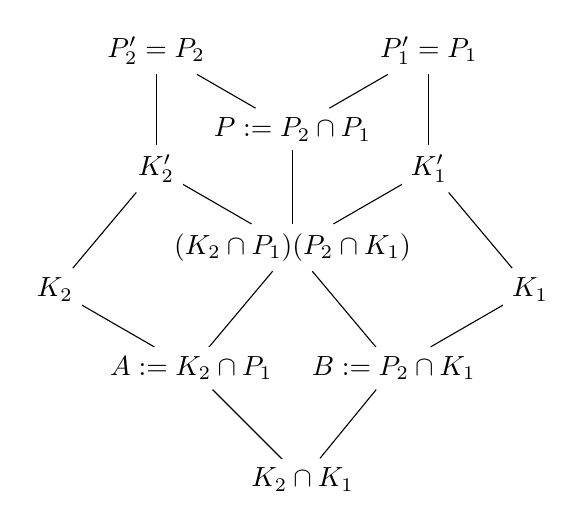
\begin{tikzpicture}
\tikzstyle{every node} = [fill = white, minimum size = 4pt]

\draw (0, 0) node (1) {$(K_2 \cap P_1) (P_2 \cap K_1)$};
\draw (1) --++ (90:1.5cm) node (2) {$P := P_2 \cap P_1$};
\draw (1) --++ (230:2cm) node(3) {$A := K_2 \cap P_1$};
\draw (1) --++ (310:2cm) node (4) {$B := P_2 \cap K_1$};
\draw (3) --++ (150:2cm) node (5) {$K_2$};
\draw (4) --++ (30:2cm) node (6) {$K_1$};
\draw (1) --++ (30:2cm) node (7) {$K_1'$};
\draw (1) --++ (150:2cm) node (8) {$K_2'$};
\draw (7) --++ (90:1.5cm) node (9) {$P_1' = P_1$};
\draw (8) --++ (90:1.5cm) node (10) {$P_2' = P_2$};
% \draw (10) --++ (90:1cm) node (11) {$P_2$};
% \draw (9) --++ (90:1cm) node (12) {$P_1$};
\draw (3) --++ (315:2cm) node (0) {$K_2 \cap K_1$};

\draw (9) --++ (2);
\draw (10) --++ (2);
\draw (5) --++ (8);
\draw (6) --++ (7);
\draw (4) --++ (0);
\end{tikzpicture}
\end{center}

In that case, $\tfrac{P}{A} \leq_U \tfrac{P_2}{K_2}$
and $\tfrac{P}{B} \leq_U \tfrac{P_1}{K_1}$.  Moreover, for every $Q \leq P$ that gives rise
to a subgroup $N_Q$ in $L \dagger M$, we have
$\tfrac{Q}{Q \cap A} \leq_U \tfrac{P}{A}$ and
$\tfrac{Q}{Q \cap B} \leq_U \tfrac{P}{B}$.  For $Q \leq P_2$ with $\tfrac{Q}{Q \cap A} \leq_U \tfrac{P_2}{K_2}$, define
\begin{align*}
  L_Q = \tfrac{P_1}{K_1} \to \tfrac{P_2}{K_2} \to \tfrac{Q}{Q \cap A}\text,
\end{align*}
the composition of the isomorphism $L$ with the inverse of the inclusion $Q \to P_2$.
Similarly, for $Q \leq P_3$ with $\tfrac{Q}{Q \cap B} \leq_U \tfrac{P_3}{K_3}$, define
\begin{align*}
  {}_QM = \tfrac{Q}{Q \cap B} \to \tfrac{P_3}{K_3} \to \tfrac{P_4}{K_4}\text,
\end{align*}
the composition of the inclusion $Q \to P_3$ with $M$.  Then, for each common $Q$, $N_Q = L_Q * {}_QM$.
Note that in this case $p_2(L_Q) = p_1({}_QM)$.  Therefore,
\begin{align*}
  L \dagger M = \kappa(L, M) \sum_{L',M'} L' \mathbin{\dot{*}} M'\text,
\end{align*}
where
\begin{align*}
  L \mathbin{\dot{*}} M = L * M\text{, if } p_2(L) = p_1(M)\text{, and } 0 \text{ else,}
\end{align*}
and the sum runs over all $L' \leq_U^2 L$ and all $M' \leq_U^1 M$.



\section{Next Step.}
\label{sec:next-step}

Now define
\begin{align*}
  \zeta_U(L) := \sum_{L' \leq_U L} L'.
\end{align*}
This one lives independently on the left and on the right sections of $L$:
if $L' \leq_U L$ then $(p_i(L'), k_i(L')) \leq_U (p_i(L), k_i(L))$ for $i = 1, 2$:
\begin{align*}
  L' = L'(\tfrac{P_1'}{K_1'}, \tfrac{P_2'}{K_2'}) \implies
  \mu_U(L, L') = \mu_U(\tfrac{P_1}{K_1}, \tfrac{P_1'}{K_1'}) \mu_U(\tfrac{P_2}{K_2}, \tfrac{P_2'}{K_2'})\text.
\end{align*}

We have
\begin{align*}
  \zeta_U(L \dagger M) = \kappa(L, M)\, \zeta_U(L) \mathbin{\dot{*}} \zeta_U(M)\text.
\end{align*}
\begin{proof}
  Splitting $\leq_U$ into $\leq_U^1$ and $\leq_U^2$,
  \begin{align*}
    \zeta_U(L) = \sum_{L' \leq_U L} L'
    = \sum_{\tfrac{P_1'}{K_1'} \leq_U \tfrac{P_1}{K_1}}
    \sum_{\tfrac{P_2'}{K_2'} \leq_U \tfrac{P_2}{K_2}}
    {}_{P_1'}L_{P_2'}.
  \end{align*}
  Thus
  \begin{align*}
    \zeta_U(L) \mathbin{\dot{*}} \zeta_U(M) &=
    \Bigl(\sum_{\tfrac{P_1'}{K_1'} \leq_U \tfrac{P_1}{K_1}}
    \sum_{\tfrac{P_2'}{K_2'} \leq_U \tfrac{P_2}{K_2}}
    {}_{P_1'}L_{P_2'}\Bigr)
    \mathbin{\dot{*}}
        \Bigl(\sum_{\tfrac{P_3'}{K_3'} \leq_U \tfrac{P_3}{K_3}}
    \sum_{\tfrac{P_4'}{K_4'} \leq_U \tfrac{P_4}{K_4}}
    {}_{P_3'}M_{P_4'}\Bigr) \\
&=
    \sum_{\tfrac{P_1'}{K_1'} \leq_U \tfrac{P_1}{K_1}}
    \sum_{\tfrac{P_4'}{K_4'} \leq_U \tfrac{P_4}{K_4}}
    \Bigl(\sum_{\tfrac{P_2'}{K_2'} \leq_U \tfrac{P_2}{K_2}}
    {}_{P_1'}L_{P_2'}
    \mathbin{\dot{*}}
        \sum_{\tfrac{P_3'}{K_3'} \leq_U \tfrac{P_3}{K_3}}
    {}_{P_3'}M_{P_4'}\Bigr) \\
&=
    \kappa(L, M)^{-1}
    \sum_{\tfrac{P_1'}{K_1'} \leq_U \tfrac{P_1}{K_1}}
    \sum_{\tfrac{P_4'}{K_4'} \leq_U \tfrac{P_4}{K_4}}
    {}_{P_1'}(L \dagger
    M)_{P_4'} \\
&=
    \kappa(L, M)^{-1}
    \zeta_U(L \dagger    M)\text,
  \end{align*}
  as desired.
\end{proof}


Define another product $\kstarhat$ via
\begin{align*}
  \zeta_U(L) \kstarhat \zeta_U(M) := \zeta_U(L \dagger M)
  = \kappa(L, M)\, \zeta_U(L) \mathbin{\dot{*}} \zeta_U(M)\text.
\end{align*}
Then
\begin{align*}
  L \kstarhat M
  &= \zeta_U(\mu_U(L)) \kstarhat \zeta_U(\mu_U(M))
    \stackrel{\text{def}}{=} \zeta_U(\mu_U(L) \dagger \mu_U(M)) \\
  &= \sum_{L',M'} \mu_U(L, L') \mu_U(M, M') \zeta_U(L' \dagger M') \\
  &= \sum_{L',M'} \mu_U(L, L') \mu_U(M, M') \kappa(L', M') \zeta_U(L') \mathbin{\dot{*}} \zeta_U(M') \\
  &= \sum_{\tfrac{P_i'}{K_i'}}
    \prod_{i=1}^4 \mu_U(\tfrac{P_i}{K_i}, \tfrac{P_i'}{K_i'})
    \kappa({}_{P_1'}L_{P_2'}, {}_{P_3'}M_{P_4'})
    \sum_{\tfrac{P_i''}{K_i''}}
    \prod_{i=1}^4 \zeta_U(\tfrac{P_i'}{K_i'}, \tfrac{P_i''}{K_i''})
    {}_{P_1''}L_{P_2''} \mathbin{\dot{*}} {}_{P_3''}M_{P_4''}
    \\
  &= \sum_{\tfrac{P_i'}{K_i'}}
    \prod_{i=2}^3 \mu_U(\tfrac{P_i}{K_i}, \tfrac{P_i'}{K_i'})
    \Size{K_2' \cap K_3'}
    \sum_{\tfrac{P_2''}{K_2''}}
    \sum_{\tfrac{P_3''}{K_3''}}
    \prod_{i=2}^3 \zeta_U(\tfrac{P_i'}{K_i'}, \tfrac{P_i''}{K_i''})
    {}_{P_1}L_{P_2''} \mathbin{\dot{*}} {}_{P_3''}M_{P_4}
    \\
  &= \sum_{\tfrac{P_i'}{K_i'}}
    \prod_{i=2}^3 \mu(P_i, P_i')
    \Size{(A \cap B) \cap (P_2' \cap P_3')}
    \sum_{Q} \zeta(P_2' \cap P_3', Q)
    L_{Q} \mathbin{\dot{*}} {}_{Q}M
    \\
  &= \sum_{Q}
    \sum_{\tfrac{P_2'}{K_2'}}
    \mu_U(\tfrac{P_2}{K_2}, \tfrac{P_2'}{K_2'})
    \zeta_U(\tfrac{P_2'}{K_2'}, \tfrac{Q}{K_2''})
    \sum_{\tfrac{P_3'}{K_3'}}
    \mu_U(\tfrac{P_3}{K_3}, \tfrac{P_3'}{K_3'})
    \zeta_U(\tfrac{P_3'}{K_3'}, \tfrac{Q}{K_3''})
    \kappa(L_Q, {}_QM)
    L_{Q} \mathbin{\dot{*}} {}_{Q}M
    \\
  &= ... \\
  &= \sum_Q \mu(P, Q) \kappa(L_Q, {}_QM) L_Q \mathbin{\dot{*}} {}_QM
\end{align*}

\section{Final Steps.}
\label{sec:final-step}

Suppose
\begin{align*}
  L \kstarhat M = \lambda^P_{A \cap B} (L * M)
\end{align*}
if $p_2(L) = p_1(M) = P$, and $0$ else.  We also assume for now that
$\lambda^P_{A \cap B} \neq 0$, i.e., that $G$ is cyclic.

For $L = \theta \colon p_1(L)/k_1(L) \to P/A$
and $M = \psi \colon P/B \to p_2(M)/k_2(M)$, set
\begin{align*}
  \lambda(L, M) &= \lambda^P_{A \cap B}, &
  \lambda(L) &= \lambda^{p_1(L)}_{k_1(L)}\text.
\end{align*}
We have $\lambda(M) = \lambda^P_B$ and $\lambda(L * M) = \lambda^{p_1(L)}_{k_1(L*M)}$.
Moreover,
\begin{align*}
  \lambda(L) / \lambda(L * M) &= \lambda^P_A / \lambda^P_{AB} = \lambda^P_{A \cap B} / \lambda^P_B
\end{align*}
implies
\begin{align*}
  \lambda(L) \lambda(M)
  = \lambda(L * M) \lambda(L, M).
\end{align*}
Note that $\lambda(L * M)$, $\lambda^P_{AB}$ and $\lambda^P_B$ in the denominators above
must not be zero.
(In general, if $\lambda(L) \lambda^P_{AB} = \lambda^P_A \lambda(L * M)$ then
\begin{align*}
  \lambda^P_A \lambda(L) \lambda(M)
  &=   \lambda(L) \lambda^P_A \lambda^P_B \\
  &=   \lambda(L) \lambda^P_{AB} \lambda^P_{A \cap B} \\
  &=   \lambda^P_A \lambda(L * M) \lambda^P_{A \cap B} \\
  &=   \lambda^P_A \lambda(L * M) \lambda(L, M),
\end{align*}
regardless \ldots)

\textbf{Intermezzo.}  On the sections of $G$, define a product
\begin{align*}
  \tfrac{P_1}{A} \kstartilde \tfrac{P_2}{B} = \tfrac{P}{AB}
\end{align*}
if $P_1 = P_2 = P$, and $0$ else.  Set $\zeta(\tfrac{P}{A}) = \sum_{\tfrac{P}{C} \geq_P \tfrac{P}{A}} \tfrac{P}{C}$.  Then
\begin{align*}
  \zeta(\tfrac{P}{A} \kstartilde \tfrac{P}{B}, \tfrac{P}{C}) =   \zeta(\tfrac{P}{A}, \tfrac{P}{C}) \cdot   \zeta(\tfrac{P}{B}, \tfrac{P}{C}),
\end{align*}
as $\tfrac{P}{C} \geq_P \tfrac{P}{A} \kstartilde \tfrac{P}{B} \iff \tfrac{P}{C} \geq_P \tfrac{P}{A}$ and $\tfrac{P}{C} \geq_P \tfrac{P}{B}$.
Moreover, if we define a new product $\star$ via
\begin{align*}
  \zeta(\tfrac{P}{A}) \star \zeta(\tfrac{P}{B}) = \zeta(\tfrac{P}{A} \kstartilde \tfrac{P}{B})\text,
\end{align*}
then
\begin{align*}
  \tfrac{P}{A} \star \tfrac{P}{B}
  & = \zeta(\mu(\tfrac{P}{A})) \star \zeta(\mu(\tfrac{P}{B}))
    = \zeta(\mu(\tfrac{P}{A}) \kstartilde \mu(\tfrac{P}{B})) \\
  & = \sum_{A',B'} \mu(\tfrac{P}{A}, \tfrac{P}{A'}) \mu(\tfrac{P}{B}, \tfrac{P}{B'}) \zeta(\tfrac{P}{A'} \kstartilde \tfrac{P}{B'}) \\
  & = \sum_{A',B'} \mu(\tfrac{P}{A}, \tfrac{P}{A'}) \mu(\tfrac{P}{B}, \tfrac{P}{B'}) \sum_{C} \zeta(\tfrac{P}{A'} \kstartilde \tfrac{P}{B'}, \tfrac{P}{C}) \tfrac{P}{C} \\
  & = \sum_C \sum_{A',B'} \mu(\tfrac{P}{A}, \tfrac{P}{A'}) \mu(\tfrac{P}{B}, \tfrac{P}{B'})
    \zeta(\tfrac{P}{A'}, \tfrac{P}{C}) \zeta(\tfrac{P}{B'}, \tfrac{P}{C}) \tfrac{P}{C} \\
  & = \sum_C \sum_{A'} \mu(\tfrac{P}{A}, \tfrac{P}{A'}) \zeta(\tfrac{P}{A'}, \tfrac{P}{C})
    \sum_{B'} \mu(\tfrac{P}{B}, \tfrac{P}{B'}) \zeta(\tfrac{P}{B'}, \tfrac{P}{C}) \tfrac{P}{C} \\
  & = \sum_C \delta_{AC} \delta_{BC} \tfrac{P}{C} = \tfrac{P}{A} \perp \tfrac{P}{B}\text.
\end{align*}
End of intermezzo.

Define $\tilde{L}:= \lambda(L) L$ and a new product $\star$ via transport of structure,
\begin{align*}
  \zeta(\tilde{L}) \star \zeta(\tilde{M}) = \zeta(\widetilde{L \kstarhat M}),
\end{align*}
where
\begin{align*}
  \zeta(\tilde{L}) = \sum_{L' \geq_P L} \widetilde{L'}\text.
\end{align*}

(Alternatively, we could first define a product $\kstartilde$ via
\begin{align*}
  \tilde{L} \kstartilde \tilde{M} = \widetilde{L \kstarhat M}
\end{align*}
which then has the property that
\begin{align*}
  L \kstartilde M = L * M
\end{align*}
if $p_2(L) = p_1(M)$ and $0$ else. Secondly, with $\zeta(L) = \sum_{L' \geq_P L} L'$, define
\begin{align*}
  \zeta(L) \star \zeta(M) = \zeta(L \kstartilde M),
\end{align*}
yielding the same structure as above.

In any case, we get
\begin{align*}
  L \star M = \delta_{AB} L * M,
\end{align*}
i.e., $L \star M = L * M$ if $p_2(L) = p_1(M)$ and $k_2(L) = k_1(M)$
(that is when the codomain of $L$ coincides with the domain of $M$:
this is composition of isomorphisms in the category which has the
sections of $G$ as its objects),
and $0$ else.

\begin{proof}
  The poset $\{ L' : L' \geq_P L \}$ is isomorphic to the poset $\{A' : P \unrhd A' \unrhd A \}$,
  that is $\zeta(L, L') = \zeta(\tfrac{P}{A}, \tfrac{P}{A'})$, where $A'= k_2(L')$.
  Similarly, $\{ M' : M' \geq_P M \}$ is isomorphic to
  $\{B' : P \unrhd B' \unrhd B \}$, with $\zeta(M, M') = \zeta(\tfrac{P}{B}, \tfrac{P}{B'})$, where $B'= k_1(M')$.
  Moreover,
  \begin{align*}
    \zeta(L \kstartilde M, N) = \zeta(\tfrac{P}{A} \kstartilde \tfrac{P}{B}, \tfrac{P}{C}) = \zeta(\tfrac{P}{A}, \tfrac{P}{C}) \cdot   \zeta(\tfrac{P}{B}, \tfrac{P}{C}),
  \end{align*}
  where $N$ is the unique group with $N \geq_P L \kstartilde M$ that factors through $\tfrac{P}{C}$, for $P \unrhd C \unrhd AB$.
  It follows that
  \begin{align*}
    L \star M &= \zeta(\mu(L)) \star \zeta(\mu(M))
= \zeta(\mu(L) \kstartilde \mu(M)) \\
  & = \sum_{L',M'} \mu(L, L') \mu(M, M') \zeta(L' \kstartilde M') \\
  & = \sum_{L',M'} \mu(L, L') \mu(M, M') \sum_{N} \zeta(L' \kstartilde M', N) N \\
  & = \sum_{A',B'} \mu(\tfrac{P}{A}, \tfrac{P}{A'}) \mu(\tfrac{P}{B}, \tfrac{P}{B'})
    \sum_C \zeta(\tfrac{P}{A'} \kstartilde \tfrac{P}{B'}, \tfrac{P}{C}) N \\
  % & = \sum_C \sum_{A',B'} \mu(\tfrac{P}{A}, \tfrac{P}{A'}) \mu(\tfrac{P}{B}, \tfrac{P}{B'})
  %  \zeta(\tfrac{P}{A'}, \tfrac{P}{C}) \zeta(\tfrac{P}{B'}, \tfrac{P}{C}) N \\
  & = \sum_C \sum_{A'} \mu(\tfrac{P}{A}, \tfrac{P}{A'}) \zeta(\tfrac{P}{A'}, \tfrac{P}{C})
    \sum_{B'} \mu(\tfrac{P}{B}, \tfrac{P}{B'}) \zeta(\tfrac{P}{B'}, \tfrac{P}{C}) N \\
    & = \sum_C \delta_{AC} \delta_{BC} N = \delta_{AB} L * M\text.
  \end{align*}
\end{proof}

\end{document}
